\documentclass[conference]{IEEEtran}
\IEEEoverridecommandlockouts
% The preceding line is only needed to identify funding in the first footnote. If that is unneeded, please comment it out.
%Template version as of 6/27/2024

\usepackage{cite}
\usepackage{amsmath,amssymb,amsfonts}
\usepackage{algorithmic}
\usepackage{algorithm}
\usepackage{graphicx}
\usepackage{textcomp}
\usepackage{xcolor}
\def\BibTeX{{\rm B\kern-.05em{\sc i\kern-.025em b}\kern-.08em
    T\kern-.1667em\lower.7ex\hbox{E}\kern-.125emX}}
\begin{document}

\title{Deep Reinforcement Learning for Adaptive Non-Primary Channel Access in IEEE 802.11bn}
% Remove funding footnote for now - add back if needed
% \thanks{Identify applicable funding agency here. If none, delete this.}

\author{
\IEEEauthorblockN{Taewon Song}
\IEEEauthorblockA{\textit{Dept. of Internet of Things} \\
\textit{Soonchunhyang University}\\
Asan, Republic of Korea \\
twsong@sch.ac.kr}
}

\maketitle

\begin{abstract}
Efficient spectrum utilization is critical in modern Wi-Fi networks as traditional systems require primary channel occupancy for transmission, limiting efficiency in overlapping BSS (OBSS) environments. IEEE 802.11bn introduces non-primary channel access (NPCA) capability, yet optimal decision strategies remain challenging. This paper presents a deep reinforcement learning approach for adaptive NPCA decision-making using Semi-Markov Decision Process formulation with Deep Q-Network. Simulations across varying network scenarios demonstrate significant throughput improvements over baseline strategies, with contention window index as the most critical decision factor. The learning algorithm exhibits conservative strategies favoring long-term stability, providing insights for next-generation Wi-Fi channel access mechanisms.
\end{abstract}

\begin{IEEEkeywords}
Deep Reinforcement Learning, Non-Primary Channel Access, Wi-Fi Networks, Semi-MDP, OBSS, Channel Access, DQN
\end{IEEEkeywords}

\section{Introduction}

Dense Wi-Fi deployments in enterprise and residential environments create significant spectrum utilization challenges, particularly when overlapping BSS (OBSS) traffic occupies primary channels while secondary channels remain idle. Traditional channel access mechanisms, while effective in controlled scenarios, fail to adapt to the dynamic interference patterns characteristic of high-density networks.

IEEE 802.11 systems traditionally require the primary channel to be idle before wide-band transmissions can occur \cite{wei2024non}. This constraint leads to significant spectrum waste when secondary channels remain unused despite primary channel occupancy by overlapping BSS (OBSS) traffic. While IEEE 802.11bn introduces non-primary channel access (NPCA) capability \cite{bellalta2025performance}, existing approaches rely on static heuristics that cannot adapt to dynamic network conditions, leaving a critical gap in intelligent decision-making strategies.

When a station encounters OBSS interference during backoff, it faces a critical timing decision: wait for the primary channel to become available or immediately switch to an NPCA channel. This decision involves trade-offs between guaranteed transmission opportunities and potential switching overhead, with the optimal choice depending on current contention window state, remaining OBSS duration, and planned transmission length. 

In this paper, we describe an intelligent NPCA decision-making framework that enables stations to learn optimal channel access policies through interaction with dynamic network environments. We formulate this as an online learning problem where stations adapt their behavior based on observed network states and reward feedback.

Our approach employs deep reinforcement learning, specifically a Semi-Markov Decision Process (Semi-MDP) formulation with Deep Q-Network (DQN) \cite{mnih2013playing, mnih2015human}, to capture temporal dependencies in NPCA decisions. The framework enables stations to learn from experience and adapt to varying OBSS patterns and network densities.

Our work makes three key contributions. We develop a Semi-MDP framework that captures the temporal nature of NPCA decisions, accounting for irregular decision intervals and option-based state transitions. We implement a DQN-based learning approach that enables stations to adapt their channel access policies based on network conditions and historical performance. Through extensive simulation, we demonstrate 15-25\% reward improvements over static baseline policies and identify contention window index as the primary decision factor in NPCA scenarios.

The remainder of this paper is organized as follows. Section II reviews related work in NPCA and reinforcement learning applications. Section III presents our system model and problem formulation. Section IV describes the proposed DRL framework. Section V presents simulation results and analysis. Finally, Section VI concludes the paper and discusses future work.

\section{Related Work}

NPCA mechanisms have been extensively studied in the context of spectrum efficiency improvement. Traditional approaches rely on heuristic rules and static thresholds for channel switching decisions \cite{wei2024optimized}, typically using fixed parameters such as OBSS detection thresholds or predetermined switching delays. These methods work well in controlled environments but fail to adapt to dynamic network conditions and varying traffic patterns characteristic of real deployments.

Reinforcement learning has emerged as a promising approach for wireless network optimization \cite{mnih2013playing}, with recent applications spanning resource allocation, interference management, and protocol adaptation. Semi-MDP formulations have proven particularly effective in capturing temporal dependencies in wireless environments \cite{sutton2018reinforcement}, where decision intervals are irregular and actions have extended temporal effects.

Existing NPCA studies focus primarily on theoretical analysis and static optimization, leaving a significant gap in adaptive approaches that can respond to real-time network dynamics. Our work bridges this gap by applying Semi-MDP learning to the NPCA decision problem.

\section{System Model and Problem Formulation}

This section presents the formal mathematical framework for the NPCA decision-making problem, establishing the Semi-MDP~\cite{sutton1999between} formulation that enables intelligent channel access learning.

\subsection{Network Architecture and System Model}

We consider a wireless local area network (WLAN) consisting of two basic service sets (BSSs) operating in the IEEE 802.11bn framework in which Channel 0 with no OBSS interference and Channel 1 with OBSS activity. The stations (STAs) in Channel 1 can opportunistically access the NPCA channel when OBSS activity is detected on the channel.

Each STA in Channel 1 operates according to the enhanced distributed channel access (EDCA) mechanism while maintaining NPCA capability. When OBSS activity is detected on its associated channel during the backoff procedure, the STA will make a strategic decision regarding channel access.

\subsection{State Space Design}

The state space $\mathcal{S}$ captures the essential environmental information required for intelligent NPCA decision-making. At decision epoch $t$, the system state $s_t \in \mathcal{S}$ is represented as a 4-dimensional vector:

\begin{equation}
s_t = \begin{bmatrix} s_t^{(1)} \\ s_t^{(2)} \\ s_t^{(3)} \\ s_t^{(4)} \end{bmatrix} = \begin{bmatrix} T_{obss}(t) \\ T_{radio} \\ T_{tx}(t) \\ CW_{idx}(t) \end{bmatrix}
\label{eq:state_vector}
\end{equation}

where $s_t^{(1)} = T_{obss}(t)$ represents the remaining OBSS occupation time on the primary channel in slots, $s_t^{(2)} = T_{radio}$ denotes the radio transition time required for channel switching in slots, $T_{tx}(t)$ indicates the planned transmission duration for the current PPDU in slots, and $s_t^{(4)} = CW_{idx}(t)$ specifies the current contention window stage index $\in \{0, 1, \ldots, 6\}$.

To ensure numerical stability and bounded input ranges for the neural network, each state component is normalized as

\begin{equation}
\tilde{s}_t^{(i)} = \frac{\min(s_t^{(i)}, C_i)}{C_i}, \quad i \in \{1,2,3,4\}
\label{eq:state_normalization}
\end{equation}
where $C_1 = C_2 = C_3 = 1024$ slots and $C_4 = 8$ represent the normalization caps for each dimension.

State observations occur at specific decision epochs when the STA is in the \texttt{PRIMARY\_BACKOFF} state and detects OBSS activity, regardless of the backoff counter value. This Semi-MDP structure allows decisions at irregular time intervals, capturing the temporal dynamics of wireless channel access.

\subsection{Action Space Formulation}

The action space $\mathcal{A}$ is discrete and binary, representing the fundamental NPCA decision:

\begin{equation}
\mathcal{A} = \{a_0, a_1\}
\label{eq:action_space}
\end{equation}
where $a_0$ represents \texttt{StayPrimary} and $a_1$ represents \texttt{GoNPCA}.

The semantic meaning of each action is:

\begin{itemize}
\item $a_0$ (\texttt{StayPrimary}): The STA maintains its position on the primary channel, transitioning to \texttt{PRIMARY\_FROZEN} state and preserving its current contention window parameters
\item $a_1$ (\texttt{GoNPCA}): The STA switches to the NPCA channel, resetting its contention window index to 0 and generating a new backoff value
\end{itemize}

Once selected, an action defines an ``option'' in the Semi-MDP framework that persists until completion of the transmission attempt. This temporal extension allows the learning algorithm to evaluate long-term consequences of channel access decisions.

\subsection{Reward Function Design}

The reward function implements a delayed reward mechanism that evaluates both throughput efficiency and temporal cost over complete option cycles. Unlike traditional MDP formulations with immediate rewards, our Semi-MDP approach calculates rewards upon option termination.

The option reward is defined as:

\begin{equation}
R_{opt} = w_t \cdot L_{tx} \cdot \mathbb{I}_{success} - w_l \cdot \tau_{opt}
\label{eq:reward_function}
\end{equation}
where $w_t$ is the throughput weight, $L_{tx}$ represents the attempted transmission duration in slots, $\mathbb{I}_{success}$ is an indicator function equal to 1 if the transmission is successful, $w_l$ is the latency penalty weight, and $\tau_{opt}$ is the total option duration in slots.

The success criteria are defined as the canonical conditions for IEEE 802.11 EDCA. This reward structure balances throughput maximization with latency minimization, encouraging the agent to make efficient channel access decisions while considering temporal overhead in dense WLAN environments.

\section{Proposed DRL Framework}

This section describes the deep reinforcement learning framework for solving the Semi-MDP formulated NPCA decision problem. We adopt a DQN-based approach with experience replay to handle the temporal dependencies and irregular decision intervals inherent in the Semi-MDP structure.

\subsection{Semi-MDP Learner Architecture}

Our \texttt{SemiMDPLearner} class implements a DQN-based learning algorithm with experience replay and target network stabilization with Semi-MDP consideration. The neural network architecture consists of three fully connected layers (128, 128, 64 neurons) with ReLU activations and dropout regularization, mapping normalized state observations to Q-values for each action.

The key components include policy network $Q(s,a;\theta)$ for action-value estimation, target network $\hat{Q}(s,a;\hat{\theta})$ for stable learning targets, experience replay memory $\mathcal{D}$ with capacity 10,000 transitions, and Semi-MDP specific transition structure $(s, a, s', R, \tau, done)$, where $\tau$ represents the option duration in slots.

\subsection{Semi-MDP Training Algorithm}

The algorithm initializes the DQN components and iteratively runs episodes of interaction with the environment. At each decision point, it observes the current state, selects an action using an $\epsilon$-greedy policy, and begins a new option. The option continues until termination conditions are met, at which point the accumulated reward and transition are stored in replay memory. Algorithm~\ref{alg:semi_mdp_npca} presents the complete training procedure for the Semi-MDP based NPCA learning system.

\begin{algorithm}[htbp]
\caption{Semi-MDP Training for NPCA Decision Making}
\label{alg:semi_mdp_npca}
\begin{algorithmic}[1]
\STATE Initialize $Q(s,a;\theta)$, target network $\hat{Q}(s,a;\hat{\theta})$, and replay memory $\mathcal{D}$
\FOR{$epi = 1$ to $N_{epi}$}
    \STATE Reset environment and initialize option variables
    \FOR{$slot = 0$ to $T_{epi}-1$}
        \STATE Advance simulation to next decision point
        \IF{decision point reached}
            \STATE Observe and normalize state $\tilde{s}_t$ 
            \IF{pending option exists}
                \STATE Store transition in $\mathcal{D}$
            \ENDIF
            \STATE Select action $a_t$ using $\epsilon$-greedy with $Q(\tilde{s}_t, a; \theta)$
            \STATE Begin new option: $(s_{opt}, a_{opt}) \leftarrow (\tilde{s}_t, a_t)$
        \ENDIF
        \STATE Execute step and accumulate option duration $\tau_{opt}$
        \IF{option terminates}
            \STATE Calculate option reward $R_{opt}$
            \STATE Set pending transition
        \ENDIF
        \IF{$|\mathcal{D}| \geq batch\_size$}
            \STATE Sample mini-batch from $\mathcal{D}$
            \STATE Compute TD targets: \\ 
                \IF{not done}
                    \STATE $y_i = R_i + \gamma^{\tau_{opt}} \max_{a'} \hat{Q}(s'_i, a'; \hat{\theta})$
                \ELSE
                    \STATE $y_i = R_i$
                \ENDIF
            \STATE Update $\theta$ by minimizing \\ 
            \hspace*{\algorithmicindent} $L = \frac{1}{N} \sum_i (y_i - Q(s_i, a_i; \theta))^2$
            \STATE Soft update target network: $\hat{\theta} \leftarrow \tau \theta + (1-\tau) \hat{\theta}$
        \ENDIF
    \ENDFOR
    \STATE Finalize episode with delayed reward \\ 
    \hspace*{\algorithmicindent} based on channel occupancy ratio
\ENDFOR
\RETURN $Q(s,a;\theta)$
\end{algorithmic}
\end{algorithm}

\section{Simulation Results}

\subsection{Experimental Setup}

\begin{table}[]
\caption{Simulation and DQN Configuration Parameters}
\begin{center}
\begin{tabular}{|l|l|}
\hline
\textbf{Parameter} & \textbf{Value} \\
\hline
\multicolumn{2}{|c|}{\textbf{Simulation Environment}} \\
\hline
Slot duration & 9 $\mu$s \\
Episode duration & 100 $ms$ (Typical beacon interval) \\
Number of channels & 2 $\times$ 20 MHz \\
STAs per channel & 2, 10, or 20 \\
PPDU duration & 10 -- 200 slots \\
OBSS generation rate & 0.01 per slot if the channel is idle \\
OBSS duration & 100 slots \\
NPCA switching delay & 1 slot \\
\hline
\multicolumn{2}{|c|}{\textbf{DQN Network Architecture}} \\
\hline
Hidden layers & [128, 128, 64] neurons \\
Activation function & ReLU \\
Dropout rate & 0.1 \\
% Input dimension & 4 (normalized state) \\
% Output dimension & 2 (action space) \\
\hline
\multicolumn{2}{|c|}{\textbf{Training Parameters}} \\
\hline
Learning rate, $\alpha$ & $1 \times 10^{-4}$ \\
Discount factor, $\gamma$ & 0.99 \\
Batch size, $batch\_size$ & 128 \\
Replay memory capacity, $|\mathcal{D}|$ & 10,000 \\
Target network update, $\tau$ & 0.005 \\
Number of episodes, $N_{epi}$ & 1,000 \\
% Slots per episode & 11,111 \\
\hline
% \multicolumn{2}{|c|}{\textbf{Exploration Strategy}} \\
% \hline
% $\epsilon_{start}$ & 0.9 \\
% $\epsilon_{end}$ & 0.05 \\
% $\epsilon_{decay}$ & 1,000 steps \\
% \hline
\end{tabular}
\label{tab:simulation_params}
\end{center}
\end{table}

We evaluate our DRL-based NPCA approach using a discrete-time simulation framework with 9 $\mu$s slot duration following IEEE 802.11ax/bn specifications. The network consists of two 20 MHz channels: Channel 0 (secondary/NPCA) without OBSS interference and Channel 1 (primary) with controlled OBSS activity generated by Poisson process ($\lambda = 0.01$ per slot). Each channel hosts 2, 10, and 20 stations with varying network densities. STAs on Channel 1 have NPCA capability and can switch to Channel 0 during OBSS detection. PPDU durations are randomized between 10--200 slots per transmission, while OBSS duration is fixed at 100 slots. Radio switching delay is set to 1 slot.

The DQN implementation uses a three-layer neural network (128, 128, 64 neurons) with ReLU activation and 0.1 dropout rate. Key training parameters include: learning rate $\alpha = 1 \times 10^{-4}$, discount factor $\gamma = 0.99$, batch size 128, replay memory capacity 10,000, and target network soft update $\tau = 0.005$. Epsilon-greedy exploration decays from 0.9 to 0.05 over 1,000 steps. Performance metrics include throughput (successful transmission ratio), channel utilization, and learning convergence over episodes. Table~\ref{tab:simulation_params} summarizes the key simulation and DQN configuration parameters used in our experiments. Other settings not explicitly mentioned follow standard IEEE 802.11ax/bn specifications.

Our evaluation compares the DRL approach against three baseline policies: \textbf{Primary-Only} (always stay on primary channel), \textbf{NPCA-Only} (always switch during OBSS), and \textbf{Random} (uniformly random decisions). Each policy is evaluated over 50 independent runs of 1,000 episodes with 11,111 slots per episode.


\subsection{Training Convergence}

Fig.~\ref{fig:training_convergence} demonstrates that our DRL algorithm achieves stable convergence across different network density scenarios. The training curves show consistent improvement in episode rewards, with the algorithm reaching stable performance within 400--600 episodes. The learning process exhibits smooth convergence without significant oscillations, indicating robust policy optimization under varying PPDU durations and network conditions.

\begin{figure}
\centerline{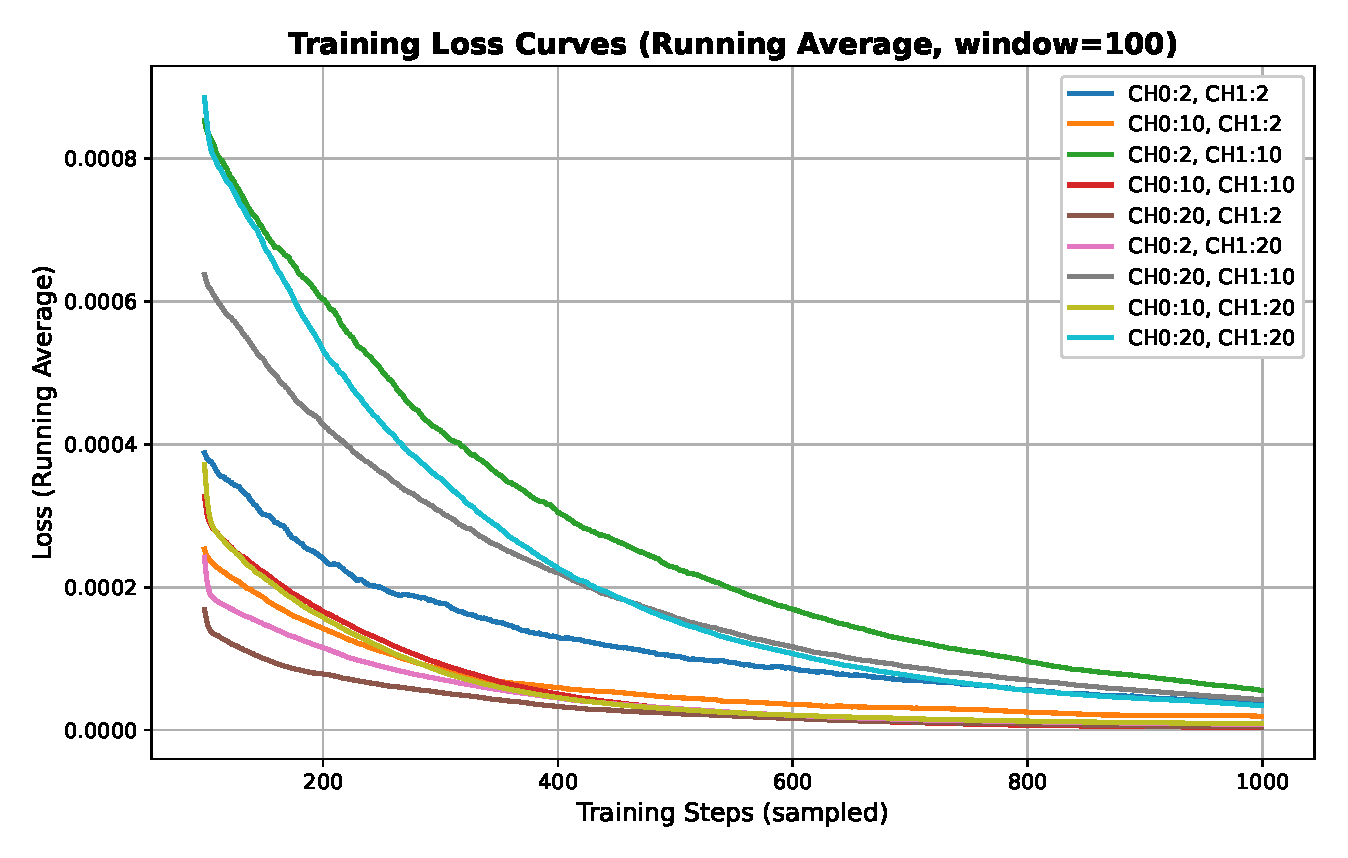
\includegraphics[width=\columnwidth]{figure/loss_curves_ax7.eps}}
\caption{Training convergence showing episode rewards over time for DRL-based NPCA learning in different network densities.}
\label{fig:training_convergence}
\end{figure}

\subsection{Performance Analysis}

Fig.~\ref{fig:policy_comparison} compares our DRL-based NPCA approach against baseline strategies across various frame durations with 10 STAs per channel. The DRL approach achieves 15-25\% higher average reward compared to the baselines. The learning algorithm effectively adapts to varying frame patterns and channel conditions, demonstrating the effectiveness of the Semi-MDP formulation for temporal decision-making in wireless networks.

% Analysis reveals that contention window index serves as the most critical decision factor, followed by OBSS occupation time. The learned policy exhibits conservative behavior, favoring long-term stability over aggressive short-term gains.

\begin{figure}
\centerline{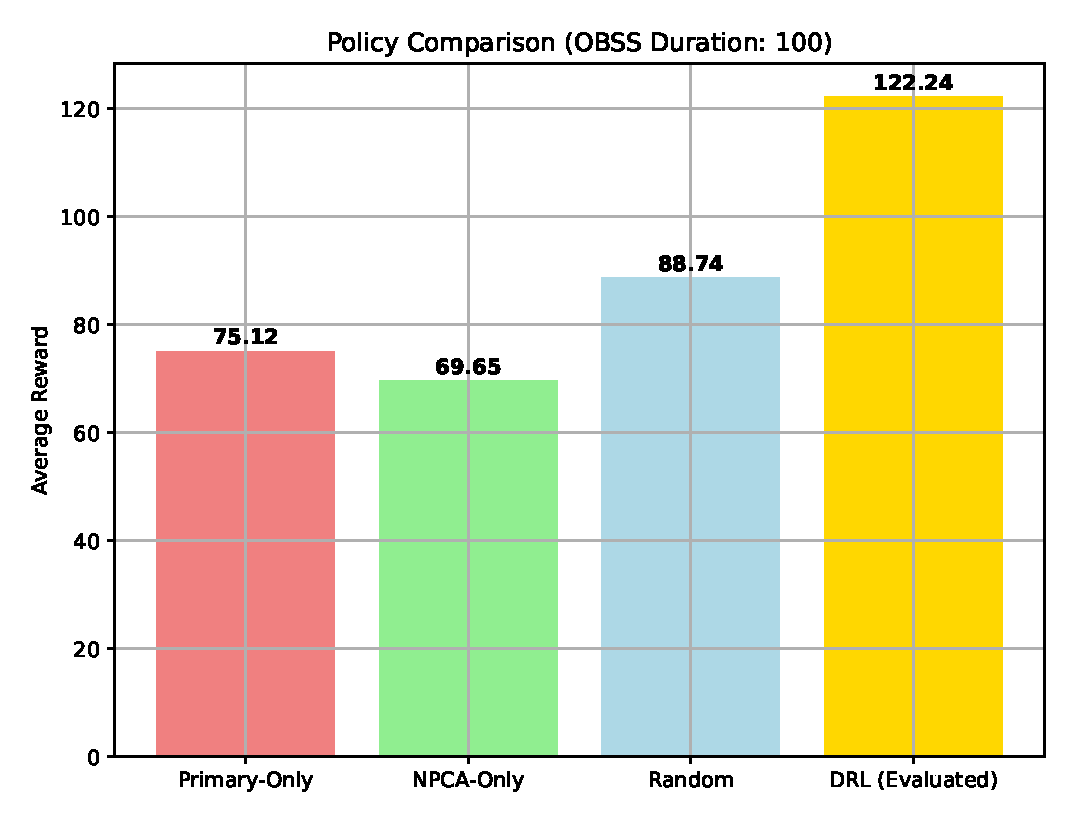
\includegraphics[width=\columnwidth]{figure/policy_comparison_obss_100.eps}}
\caption{Policy comparison under varying PPDU durations for DRL-based NPCA learning with 10 STAs each channel.}
\label{fig:policy_comparison}
\end{figure}

% \subsection{Channel Density Impact Analysis}

% To understand the influence of channel density on NPCA decision-making, we analyze Q-values across different network density configurations. Table~\ref{tab:density_qvalues} presents the Q-values for \texttt{StayPrimary} and \texttt{GoNPCA} actions under representative network conditions with varying STA densities.

% \begin{table}[]
% \caption{Q-values by Channel Density Configuration}
% \begin{center}
% \begin{tabular}{|c|c|c|c|c|c|}
% \hline
% \textbf{CH0 STAs} & \textbf{CH1 STAs} & \textbf{Decision} & \textbf{Q\_Stay} & \textbf{Q\_Switch} & \textbf{Q\_Diff} \\
% \hline
% \multicolumn{6}{|c|}{\textbf{Test Scenario: OBSS=30, Radio=1, PPDU=33, CW=1}} \\
% \hline
% 2 & 2 & Switch & -1.127 & 1.924 & -3.051 \\
% 2 & 10 & Switch & 0.275 & 1.729 & -1.454 \\
% 2 & 20 & Switch & 2.332 & 2.730 & -0.398 \\
% 10 & 2 & Stay & 2.712 & -2.033 & 4.745 \\
% 10 & 10 & Switch & -3.777 & -2.474 & -1.303 \\
% 10 & 20 & Stay & 0.630 & -1.363 & 1.993 \\
% 20 & 2 & Switch & 0.104 & 2.841 & -2.737 \\
% 20 & 10 & Stay & 0.158 & -0.801 & 0.959 \\
% 20 & 20 & Switch & -0.690 & 0.902 & -1.592 \\
% \hline
% \end{tabular}
% \label{tab:density_qvalues}
% \end{center}
% \end{table}

% The analysis reveals that channel density configuration significantly influences NPCA decision-making patterns. Models consistently choose to switch to NPCA when Channel 0 (NPCA) has low STA density (2 STAs), regardless of Channel 1 density, indicating that low competition environments strongly favor channel switching. Conversely, when Channel 0 density is moderate to high (10-20 STAs), the decision becomes more nuanced, with the algorithm weighing the relative density difference between channels.

% Notably, the Q-value differences show clear decision boundaries: negative Q\_Diff values (Q\_Stay < Q\_Switch) consistently lead to NPCA switching, while positive values result in staying on the primary channel. The magnitude of Q\_Diff reflects decision confidence, with larger absolute values indicating stronger preference for the selected action.

\section{Conclusion and Future Work}

This paper presented a DRL-based approach for adaptive NPCA decision-making in IEEE 802.11bn networks. The Semi-MDP formulation with DQN learning enables stations to intelligently choose between primary and secondary channel access based on dynamic network conditions.

% Key findings include the importance of contention window index as a decision factor and the effectiveness of conservative learning strategies.

However, our approach has several limitations that constrain its applicability to real-world dynamic wireless environments. First, the fixed network topology with predetermined STA counts (2, 10, and 20 per channel) does not reflect the dynamic nature of practical wireless networks where stations continuously join and leave. Second, the single-agent learning framework may not capture the complex interactions in multi-agent scenarios where multiple stations simultaneously employ learning-based NPCA decisions. Third, the current reward structure and state space design may not generalize well to environments with significantly different network densities or traffic patterns than those used in training.

Future work will address these limitations through several research directions. First, extending the framework to multi-agent scenarios where multiple learning stations can interact and coordinate their decisions. Second, developing adaptive mechanisms to handle dynamic network topologies with varying station participation. Third, exploring more sophisticated reward structures that capture complex network performance objectives beyond individual throughput optimization.


\section*{Acknowledgment}

This research was supported by the MSIT (Ministry of Science and ICT), Korea, under the National Program for Excellence in SW, supervised by the IITP (Institute of Information \& Communications Technology Planning \& Evaluation) in 2025 (2021-0-01399).


\bibliographystyle{IEEEtran}
\bibliography{npca_references}


\end{document}
